\section{结果分析}
\label{sec:results}
表~\ref{tab:results}展示结果表格式，“待填”应替换为实际计算值。
结合式~\eqref{eq:objectives}解释目标取舍、方案选择依据与约束满足情况。
\begin{table}[htbp]
  \centering
  \caption{方案比较（结果待填写）}
  \label{tab:results}
  \begin{tabular}{@{}lccc@{}}
    \toprule
    方案 & 碳排/(kg CO$_2$e/m$^3$) & 成本/(元/m$^3$) & 强度/MPa\\
    \midrule
    基准方案 & 待填 & 待填 & 待填\\
    折中方案 & 待填 & 待填 & 待填\\
    \bottomrule
  \end{tabular}
\end{table}

图~\ref{fig:pareto-example}取自随附的三目标合成数据演示，仅用于展示插图格式。
横纵轴分别为碳排放与合成强度，圆点颜色表示成本。使用时替换图片及说明。
\begin{figure}[htbp]
  \centering
  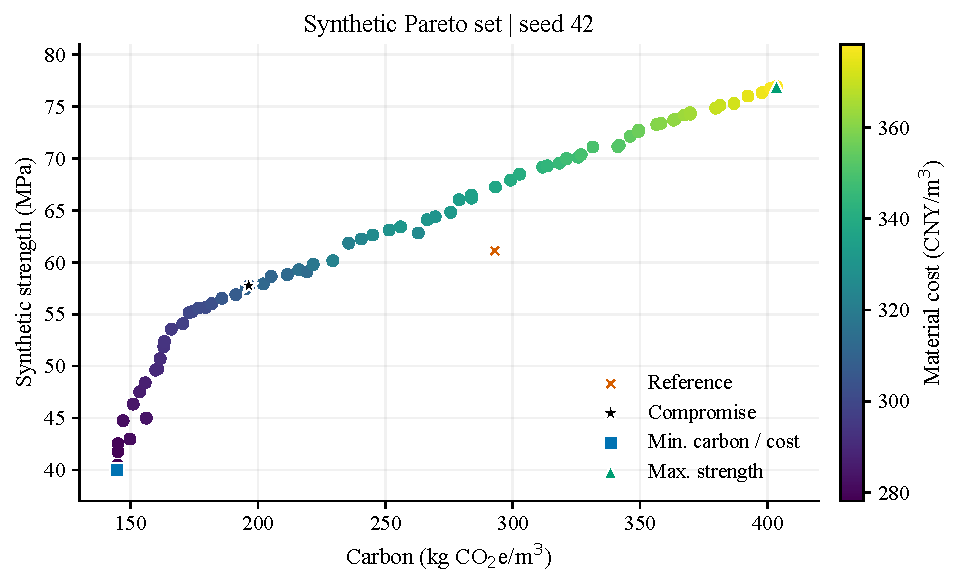
\includegraphics[width=0.88\linewidth]{figures/pareto.pdf}
  \caption{合成数据演示的 Pareto 解集（插图示例）}
  \label{fig:pareto-example}
\end{figure}
